\documentclass[]{article}

% Get better typography
\usepackage[protrusion=true,expansion=true]{microtype}		

% For algorithms
\usepackage[boxruled,linesnumbered,vlined,inoutnumbered]{algorithm2e}
\SetKwInOut{Parameter}{Parameters}

% For basic math, align, fonts, etc.
\usepackage{amsmath}
\usepackage{amsthm}
\usepackage{amssymb}
\usepackage{mathtools}
\usepackage{mathrsfs}
\usepackage{rotating}
\usepackage{gensymb} % For \degree

\usepackage{enumitem} %for enumerating with letters

\newtheorem{defn}{Definition}[]
\newtheorem{thm}{Theorem}[]
\newtheorem{claim}{Claim}[]
\newtheorem{lemma}{Lemma}[]
\newtheorem{prop}{Property}[]
\newtheorem{ass}{Assumption}[]
\newtheorem{cor}{Corollary}[]

\DeclareMathOperator*{\argmin}{arg\,min}
\DeclareMathOperator*{\argmax}{arg\,max}

\usepackage{courier} % For \texttt{foo} to put foo in Courier (for code / variables)
\usepackage{lipsum} % For dummy text

% For images
\usepackage{graphicx}
\usepackage{subcaption}
\usepackage[space]{grffile} % For spaces in image names

% For bibliography
\usepackage[round]{natbib}

% For color
\usepackage{xcolor}
\definecolor{light-grey}{rgb}{0.95,0.95,0.95}
\definecolor{dark-red}{rgb}{0.4,0.15,0.15}
\definecolor{dark-blue}{rgb}{0,0,0.7}

% For questions and answers
\usepackage[framemethod=tikz]{mdframed}
\newtheorem{question}{Question}
\mdfdefinestyle{que}{
  linecolor=dark-blue,
  backgroundcolor=white!20,
}
\surroundwithmdframed[style=que]{question}
\newtheorem{answer}{Answer}
\mdfdefinestyle{ans}{
  linecolor=dark-red,
  backgroundcolor=white!20
  % , rotatebox
}
\surroundwithmdframed[style=ans]{answer}
\usepackage{environ}
\NewEnviron{Answer}
{%
\noindent
\rotatebox[origin=c]{180}{%
\noindent
\begin{minipage}[t]{\linewidth}
\begin{answer}
\BODY
\end{answer}%
\end{minipage}%
}%
}%

% Only show sections in table of contents and rename
\setcounter{tocdepth}{2}
\renewcommand{\contentsname}{Table of Contents}

% For links (e.g., clicking a reference takes you to the phy)
\usepackage{hyperref}
\hypersetup{
    colorlinks, linkcolor={dark-blue},
    citecolor={dark-blue}, urlcolor={dark-blue}
}

%-------------------------
%	BEGIN DOCUMENT / TITLE
%-------------------------

\begin{document}

%\maketitle
%\hrulefill
%-----------------
%	Homework 1
%-----------------
\newpage
\begin{center}
    \begin{Large}
    CMPSCI 687 Homework 1
    \end{Large}
    \\
    Due September 19, 2019, 11:55pm Eastern Time
\end{center}
\addcontentsline{toc}{subsection}{\textbf{Homework 1}}

\noindent {\bf Instructions: } This homework assignment consists of a written portion and a programming portion. While you may discuss problems with your peers (e.g., to discuss high-level approaches), you must answer the questions on your own. Submissions must be typed (hand written and scanned submissions will not be accepted). You must use \LaTeX. The assignment should be submitted on Gradescope as PDF with marked answers via the Gradescope interface. The source code should be submitted via the Gradescope programming assignment as a .zip file. Include with your source code instructions for how to run your code. You \textbf{must} use Python 3 for your homework code. You may not use any reinforcement learning or machine learning specific libraries in your code, e.g., TensorFlow or PyTorch (you may use libraries like numpy and matplotlib though). The automated system will not accept assignments after 11:55pm on September 19. The tex file for this homework can be found \href{https://people.cs.umass.edu/~pthomas/courses/CMPSCI_687_Fall2019/hw1Source.tex}{here}.


\section*{Part One: Written (63 Points Total)}
\begin{enumerate}
    \item (Your grade will be a zero on this assignment if this question is not answered correctly) Read the class syllabus carefully, including the academic honesty policy. To affirm that you have read the syllabus, type your name as the answer to this problem. \\

    \textbf{Answer:} Hanqing Li
    %
    \item (15 Points) Given an MDP $M=(\mathcal S, \mathcal A, P, d_R, d_0, \gamma)$ and a fixed policy, $\pi$, the probability that the action at time $t=0$ is $a \in \mathcal A$ is:
    \begin{equation}
        \Pr(A_0=a)=\sum_{s \in \mathcal S} d_0(s) \pi(s,a).
    \end{equation}
    Write similar expressions (using only $\mathcal S,\mathcal A,P,R,d_0,\gamma$, and $\pi$) for the following problems.\\
    
    \textbf{Hints and Probability Review:}
    \begin{itemize}
        \item \textbf{Write Probabilities of Events:} In some of the probability hints below that are not specific to RL, we use expressions like $\Pr(a|b)$, where $a$ and $b$ are events.  Remember that in the RL notation used for this class, the values of $\Pr(s_0)$, $\Pr(a_0)$, $\Pr(A_0)$, or $\Pr(A_0 | S_0)$ are all undefined, since those are simply states, actions, or random variables (not events).  Instead, we must write about the probabilities of events.  For example: $\Pr(A_0 = a_0)$ or $\Pr(A_0 = a_0 | S_0 = s_0)$.
        %
        \item \textbf{Bayes' Theorem:} $\Pr(a|b) = \frac{\Pr(b|a) \Pr(a)}{\Pr(b)}$. This is useful for dealing with conditional probabilities $\Pr(a|b)$, where event $a$ occurs before event $b$.  For example, it is often difficult to work with an expression like $\Pr(S_0 = s_0 | A_0 = a_0)$, but much easier to deal with the 3 terms in $\frac{\Pr(A_0 = a_0 | S_0 = s_0) \Pr(S_0 = s_0)}{\Pr(A_0 = a_0)}$.
        %
        \item \textbf{The law of total probability:} For event $a$, and a set of events $\mathcal{B}$,
        $$\Pr(a) = \sum_{b \in \mathcal B} \Pr(b) \Pr(a|b)$$ See the example below for several useful applications of this property.
        \item \textbf{``Extra'' given terms:} Remember that when applying laws of probability, any ``extra'' given terms stay in the result.  For example, applying the law of total probability: $$\Pr(a|c,d) = \sum_{b \in \mathcal B} \Pr(b|c,d) \Pr(a|b,c,d)$$
        %
        \item \textbf{Example problem:} The probability that the state at time $t = 1$ is $s \in \mathcal S$. 
        \begin{align}
        \Pr(S_1 = s) =& \sum_{s_0 \in \mathcal S} \Pr(S_0 = s_0) \Pr(S_1 = s | S_0 = s_0) \\
        %
        =& \sum_{s_0\in \mathcal S} d_0(s_0) \Pr(S_1 = s | S_0 = s_0)\\
        %
        =& \sum_{s_0\in \mathcal S} d_0(s_0) \sum_{a_0\in \mathcal A} \Pr(A_0 = a_0 | S_0 = s_0)\\
        &\times \Pr(S_1 = s | S_0 = s_0, A_0 = a_0)\\
        %
        =& \sum_{s_0\in \mathcal S} d_0(s_0) \sum_{a_0\in \mathcal A} \pi(s_0, a_0) P(s_0, a_0, s).
        \end{align}
    \end{itemize}
    %
    \textbf{Problems:}\\
    \begin{enumerate}[label=\Alph*]
        \item The probability that the action at time $t=3$ is either $ a \in \mathcal A$ or $a' \in \mathcal A$, with $a \ne a'$.
        \\
        \textbf{Answer: }\\
        \begin{align}
            \Pr(A_3=a)+Pr(A_3=a')\\
            %
            =& \sum_{s_3\in \mathcal S} Pr(S_3=s_3) Pr(A_3=a|S_3=s_3)+\sum_{s_3\in \mathcal S} Pr(S_3=s_3) Pr(A_3=a'|S_3=s_3)\\
            %
            =& \sum_{s_3\in \mathcal S} Pr(S_3=s_3) \pi(s_3,a)+\sum_{s_3\in \mathcal S} Pr(S_3=s_3) \pi(s_3,a')
        \end{align}

        \item The expected reward at time $t=6$ given that the action at time $t=5$ is $a \in \mathcal A$ and the state at time $t=4$ is $s\in \mathcal S$.
        \\
        \textbf{Answer: }\\
        $\mathbf{E}[R_6|A_5=a,S_4=s] $
        \item The probability that the action at time $t=16$ is $a' \in \mathcal A$ given that the action at time $t=14$ is $a \in \mathcal A$, and the state at time $t=15$ is $s \in \mathcal S$.
        
        \item The probability that the initial state was $s \in \mathcal S$ given that the action at time $t=1$ is $a' \in \mathcal A$. 
        
        \item The expected reward at time $t=3$ given that the initial state is $s \in \mathcal S$, the state at time $t=3$ is $s' \in \mathcal S$, and the action at time $t=4$ is $a' \in \mathcal A$.
       
    \end{enumerate}
    
    \item (3 Points) In 687-Gridworld, if we changed how rewards are generated so that hitting a wall (i.e., when the agent would enter an obstacle state, and is placed back where it started) results in a reward of $-10$, then what is $\mathbf{E}[R_t|S_t=17,A_t=\text{AL}, S_{t+1}=17]$?\\
    \textbf{Answer:}\\
    $\mathbf{E}[R_t|S_t=17,A_t=\text{AL}, S_{t+1}=17]\\
    =0.8*(-10)+0.1*0\\
    =-8$


    \item (2 Points) How many deterministic policies are there for an MDP with $|\mathcal S|< \infty$ and $|\mathcal A|<\infty$? (You may write your answer in terms of $|\mathcal S|$ and $|\mathcal A|$).\\
    \textbf{Answer:}\\
    $|\mathcal S|^{|\mathcal A|}$
    
    
    \item (5 Points) Give an example of an MDP with $|\mathcal S| < \infty, |\mathcal A| = \infty$, and $\gamma < 1$ such that an optimal policy \emph{does not} exist. Give an example of an MDP with $|\mathcal S| = \infty, |\mathcal A| < \infty$, and $\gamma < 1$ such that an optimal policy exists.\\
    \textbf{Answer:}\\
    Consider a MDP with finite states with infinite actions connect between each other, and for ever actions, the reward $R_t>1$. In this situation, there is no optimal policy since that there is no maximal objective $J$.\\
    Consider a MDP which has infinite states (like the states includes the time), the agent receives rewards $R_t<1$ for every action it takes. Then the objective function can have a maximum value since it will finally constraint because $\gamma<1$.
    
    \item (3 Points) Read about the Pendulum domain, described in Section 5.1 of \href{https://homes.cs.washington.edu/~todorov/courses/amath579/reading/Continuous.pdf}{this} paper (Reinforcement Learning in Continuous Time and Space by Kenji Doya). Consider a variant where the initial state has the pendulum hanging down with zero angular velocity always (a deterministic initial state where the pendulum is hanging straight down with no velocity) and a variant where the initial angle is chosen uniformly randomly in $[-\pi,\pi]$ and the initial velocity is zero. Which variant do you expect an agent to require more episodes to solve? Why? Note: We did not talk about the complexity of solving MDPs in class yet---we want you to provide your best guess here.
    \\
    \textbf{Answer:}\\
    I expect that the variant which initial state is chosen randomly would require less episodes to solve, and the variant which initial state with pendulum hanging down will take more episodes to solve. For a learning agent, it may act randomly at the very beginning. The initial state with random angle can make the agent experience more kinds of states, which would be difficult to enter if the initial state is hanging down.

    \item (1 Point)  How many episodes do you expect an agent should need in order to find near-optimal policies for the gridworld and pendulum domains? 
    %
    Note: We did not talk about the complexity of solving MDPs in class yet---we want you to provide your best guess here. 
    \\
    \textbf{Answer:}\\
    For gridworld environment, I suppose an agent which can learn from environment may take about tens of episodes to solve the problem, since the obstacles and waters are steady and never change. For pendulum problem, I suppose the agent may take longer time to solve, since the high state is not stable, and has more probability to fail if agent do anything wrong. So maybe about 100 episodes to solve this problem.

    \item (5 Points) Select a problem that we have not talked about in class, where the agent does not make Markovian observations about the world around it. Describe how the environment for this problem can be formulated as an MDP by specifying $(\mathcal S, \mathcal A, P, [d_r\text{ or } R], d_0, \gamma)$ (your specifications of these terms may use English rather than math, but be precise). 
    \\
    \textbf{Answer:}\\
    Consider a robot which is designed to build a wall. The state can be defined as the position of every brick, which is influnced by all the previous state. $\mathcal A$ can be defined as the position of the brick the robot going to put. $P$ can be defined as the transition state after the robot put a brick on a specific position. $R$ is given after every step by estimating the stability of the wall after this step. 
    
    \item (5 Points) We refer to the discounted sum of rewards, $\sum_{t=0}^\infty \gamma^t R_t$, as the \emph{return}. Let an MDP exist such that it has two optimal policies. Can the expected value of their returns differ? If so, give an example. If not, explain why. Can the variance of their returns differ? If so, give an example. If not, explain why.\\
    \textbf{Answer:}\\
    For two optimal policies, the expected value cannot be different. The definition of optimal policy given that an optimal policy can maximize $J(pi)$, which is the expectation of the sum of all discounted rewards obtained at every step. Since we have 2 different optimal policy, so they should both have the same expectation. \\
    The variance of their returns can be different. Consider a gridworld problem with $gamma<1$ which has a water state between the start state and the end state. Any other path to the goal state without entering water state would be longer than the path through the water. The agent can choose to take the long way, spend more time, and get a lower final rewards at the goal state. Or the agent can choose to get through the water area, where it would receive a penalty but can reach the goal earlier and get a higher rewards. The final rewards the agent get in these two ways can be the same, but their variance of returns differ.
    
    \item (2 Points) Consider the one state MDP where in $s_0$ there are three actions, $a_0$, $a_1$, $a_2$, and all actions transition to $s_\infty$ with probability $0.5$ and stay in $s_0$ otherwise. The reward for taking actions $a_0$, $a_1$ are drawn from the uniform distribution on $[0,1]$ and the normal distribution $\mathcal{N}(0.5,1)$, respectively. The reward for $a_3$ is always $0.25$. What are all the optimal policies of this MDP? \\
    \textbf{Answer:}\\
    Take both $a_0$ and $a_1$ at state $s_0$ are optimal policies.
    
    %
    \item (2 Points) Read the Wikipedia page on \href{https://en.wikipedia.org/wiki/Markov_chain}{Markov chains}. A state in a \emph{Markov chain} is \emph{irreducible} if it is possible to get to any state from any state. An MDP is \emph{irreducible} if the Markov chain associated with every deterministic policy is irreducible. A state in a \emph{Markov chain} has \emph{period} $k$ if every return to the state must occur in multiples of $k$ time steps. More formally,
    $$
    k=\operatorname{gcd}\{t>0: \Pr (S_t=s|S_0=s)>0\}.
    $$
    %
    A Markov chain is \emph{aperiodic} if the period of every state is $k=1$. Can an MDP be aperiodic and \emph{not} irreducible? If so, give an example. If not, explain your reasoning. \\
    \textbf{Answer:}\\
    A MDP can be aperiodic and not irreducible. Consider a mountain car problem which the car starts from a very high platform and enter the valley. The state can be defined as the position and velocity of the car $s(x,v)$, and the action is "accelerate towards left", "accelerate towards right" or "nothing". The power of the car cannot support the car to go back to the start point. In this situation, the start state cannot occur after the car's leaving, thus it is not irreducible. And assume that the policy agent chose to accelerate towards the velocity direction and reach the goal state directly, then there is no period exists in this MDP, and every state is aperiodic.
    
   
    \item (5 Points) The state of a Markov chain is \emph{positive recurrent} if the expected time until the state recurs is finite. A Markov chain is \emph{positive recurrent} if all states are positive recurrent. Give an example of an MDP with $|S|>2$ states that is positive recurrent and aperiodic. For any number of states $|S|$, can you think of a simple way of defining state transitions such that the MDP is positive recurrent and aperiodic? Explain your methodology (a picture might be useful). \\
    \textbf{Answer:}\\
    Consider a MDP whose states consist a loop one-by-one. Among them there is a transition from state $s_0$ to state $s_0$. This MDP is positive recurrent since the expectation time for $s_0$ continuely transits to $s_0$ is finite. But the period of the recurrent is not stable, depends on if and how many continuous time step that $s_0$ transits to $s_0$.
    
    \item (1 point) Let a tabular policy representation be used to represent stochastic policies for an MDP with $n$ states and $m$ actions. What is the sum of every element in the matrix representation of this policy? Why?\\
    \textbf{Answer:}\\
    Since the policy is stochastic, then the sum of probility over all the actions in any state would be 1. Since there are $n$ states, then the sum of every matrix should be $n$.
   
    
    \item (2 Points) Describe a real-world problem and how it can be reasonably modeled as an MDP where $R_t$ is \emph{not} a deterministic function of $S_t, A_t,$ and $S_{t+1}$, and is not a bandit problem. \\
    \textbf{Answer:}\\
    Assume that a drone is required to take a package to a specific place. Define the state using the drone's height $h$ and the distance to the destination $x$ such that state $s(x,h)$, and the action is {take off,landing,move}. Suppose $S_t$ is that the drone just above the target, $S_t+1$ is drone stopped on target position, and $A_t$ is landing. Consider the situation where the drone landed too fast and destroyed the package. Though drone is still in $S_t+1$, but the rewards it received should be negative.
    
    
    \item (2 Points) If you know $(\mathcal S, \mathcal A, P, R, d_0, \gamma)$, can you derive $d_R$? Prove your answer is correct. \\
    \textbf{Answer:}\\
    $d_R$ cannot be derived. As definition, $d_R$ is a conditional distribution over $R_t$ given $S_t$, $A_t$, $S_t+1$. $R_t$ is a sample of $d_R$ given $S_t$, $A_t$. We cannot derive the probability distribution from samples.
    
    \item (2 Points) If you know $(\mathcal S, \mathcal A, P, d_R, d_0, \gamma)$, can you derive $R$? Prove your answer is correct. \\
    \textbf{Answer:}\\
    Yes. According to the definition of $R$, $R(s,a)=\mathbf{E}[R_t|S_t=s,A_t=a]$, where $R_t$ can be obtained by sampling $d_R$ given $S_t$, $A_t$, $S_t+1$.
    
    \item (2 Points) Describe a real-world problem and how it can be reasonably modeled as an MDP where $R_t$ is a deterministic function of $S_t$.\\
    \textbf{Answer:}\\
    Consider a robot trying to open a door using handle. The state is defined as the angle the handle was turned, and the reward are given according to the angle of the handle turned at every time step. Further the handle was turned, larger the reward the agent would get.

    \item (2 Points) Describe a real-world problem and how it can be reasonably modeled as an MDP where the reward function, $R$, would \emph{not} be known. \\
    \textbf{Answer:}\\
    Consider an agent trying to allocate more memory previously to a server in case of a possible peak of visiting requests. The rewards can never be sure until the peak arrives or does not arrive at time $t$. Only then the rewards of agent's allocation action can be rewarded.
    
    \item (2 Points) Describe a real-world problem and how it can be reasonably modeled as an MDP where the transition function, $P$, would be known.\\
    \textbf{Answer:}\\
    Consider a robot learning to move towards a target in a plain and steady environment. The state is defined as the distance between the target, the actions that the robot can take is "move" or "stop". In 1 time step, the robot can move 1 unit distance if it chose to move. In this case, the transition function $P$ would be known.
    
    \item (2 Points) Describe a real-world problem and how it can be reasonably modeled as an MDP where the transition function, $P$, would \emph{not} be known.\\
    \textbf{Answer:}\\
    Consider a cleanning robot trying to cover every corner of the room. The state is defined as its coordination in this room, and the robot can only observe the environment close to it. If the robot trying to move to another coordination, it may hit a desk or some other obstacles and cannot enter that state. In this situation, the transition function $P$ is not known.
    
\end{enumerate}

\section*{Part Two: Programming (25 Points Total)}

\noindent\textbf{More-Watery 687-Gridworld.} For this assignment, we will be working with a slightly modified version of the 687-Gridworld domain described in class and in the class notes. In this new Gridworld, called More-Watery Gridworld, there are two extra water states located in state 7 and state 17, as shown in Figure \ref{fig: watery gridworld}. Implement More-Watery Gridworld. 

\textbf{Codebase.} We have provided a template for programming the homework on the github repository for this class located  \href{https://github.com/bmetevier/rl-framework-687-public}{here}. You do \emph{not} need to use this template for the assignment. After the due date for this assignment, an example will be posted on this site. 

\begin{figure}[h!!!]
    \centering
	[Image omitted]
    %\includegraphics[width=1\textwidth]{watery_gridworld.pdf}
    \caption{A more watery version of 687-Gridworld. Water states are located in state 7, state 17, and state 21.}
    \label{fig: watery gridworld}
\end{figure}

\begin{enumerate}[label=\Alph*]
    \item (5 Points) Have the agent uniformly randomly select actions. Run $10,\!000$ episodes. Report the mean, standard deviation, maximum, and minimum of the observed discounted returns. \\
    \textbf{Answer: }\\
    The result is shown below:\\
        Mean: -8.18\\
        Standard Deviation: 6.52\\
        Maximum: 3.87\\
        Minimum: -43.98\\
        Random Seed: 38294238.80
    
    \item (5 Points) Find an optimal policy (you may do this any way you choose, including by reasoning through the problem yourself). Report the optimal policy here. Comment on whether it is unique. \\
    \textbf{Answer: }\\
    Optimal policy: For all the state in the upper bound, take action "Move Right". For all the states in the right bound, take action of "Move Down". If agent in any other states, then have 0.5 probability of moving right, and 0.5 probability of moving down. \\
    This optimal policy may be unique, since the agent have the possibility to "get confused" and "veer right" or "veer left", which means the movement can not be guaranteed only by the policy agent chose. Thus, if the policy drives agent leave the upper and right boundary, the probability of agent step into water area increases, which will reduce the expectation of reward agent can reach. 
    \item (5 Points) Run the optimal policy that you found in the previous question for $10,\!000$ episodes. Report the mean, standard deviation, maximum, and minimum of the observed discounted returns.\\
    \textbf{Answer: }\\
    The result is shown below:\\
        Mean: 1.61\\
        Standard Deviation: 4.71\\
        Maximum: 4.30\\
        Minimum: -36.31\\
        Random Seed: 38294238.80

    \item (5 Points) The distribution of returns is often not normal, thus it cannot be fully characterized by its mean and standard deviation. To provide more information about the performance, the empirical distribution of returns can be reported.
    For a random variable, $X$, its \textit{cumulative distribution function} (CDF), $F_X$, is defined as $F_X(x) \coloneqq \Pr(X \le x)$. The empirical CDF, $\hat F$, for a sequence of $n$ samples of $X$, $X_1,\dotsc,X_n$ is given by the function
    %
    \begin{equation*}
        \hat F_n(x) \coloneqq \frac{1}{n} \sum_{i=1}^n \mathbf{1}_{X_i \le x},
    \end{equation*}
    %
    where $X_i$ is the $i^\text{th}$ sample of $X$ and $\mathbf{1}_A$ is the indicator function of an event $A$, i.e., $\mathbf{1}_A=1$ if $A$ is true and $0$ otherwise. 
    
    The quantile function, also referred to as the inverse CDF, is the function $Q(\tau) \coloneqq \inf \{ x \in \mathbb{R} \colon \tau \le F_X(x) \}$ for $\tau \in (0,1)$. The empirical quantile function, $\hat Q$, can be constructed by considering the order statistics, $Z_i$, the sorted samples of $X_i$ such that $Z_1 \le Z_2 \le \dotsc \le Z_n$. The empirical quantile function is given by
    %
    \begin{equation*}
        \hat Q(\tau) \coloneqq Z_{\lfloor (n+1)\tau \rfloor}.
    \end{equation*}
    %
    Both the CDF and quantile functions capture all the information about a random variable, but for plotting purposes the quantile function is often preferred. This is because we are interested in maximizing returns, so the quantile function has a more natural interpretation as higher is better. 
    
    Plot the distribution of returns for both the random policy and the optimal policy using $10,\!000$ trials each. You must clearly label each line and axis. Additionally, report the random seed used for the experiments. \\
    \textbf{Answer: }\\
    Random Seed: 38294238.80\\
    The plotted result is shown in Figure 2 and Figure 3\\
    \begin{figure}
    \begin{minipage}[t]{0.5\textwidth}
    \centering
    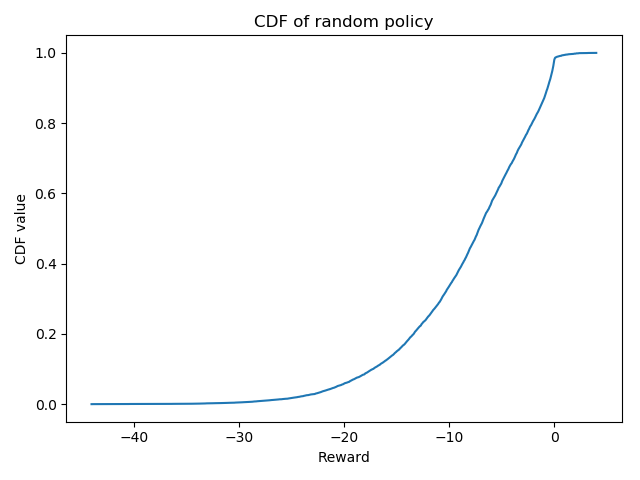
\includegraphics[height=4.5cm,width=6cm]{fig/CDF_random.jpg}
    \end{minipage}
    \begin{minipage}[t]{0.5\textwidth}
    \centering
    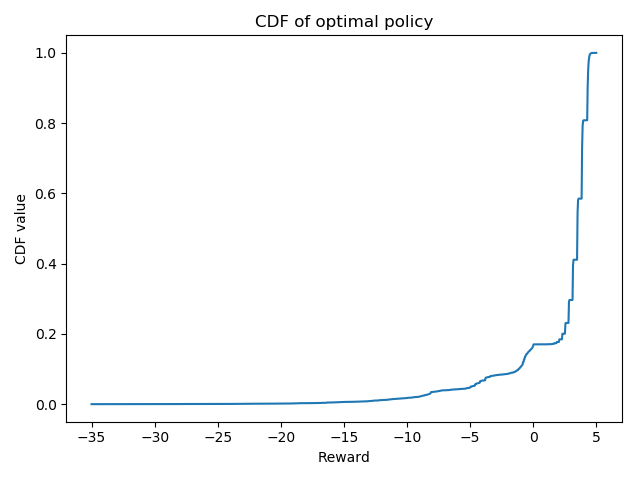
\includegraphics[height=4.5cm,width=6cm]{fig/CDF_optimal.jpg}
    \end{minipage}
    \caption{CDF of different policy}
    \end{figure}

    \begin{figure}
    \begin{minipage}[t]{0.5\textwidth}
    \centering
    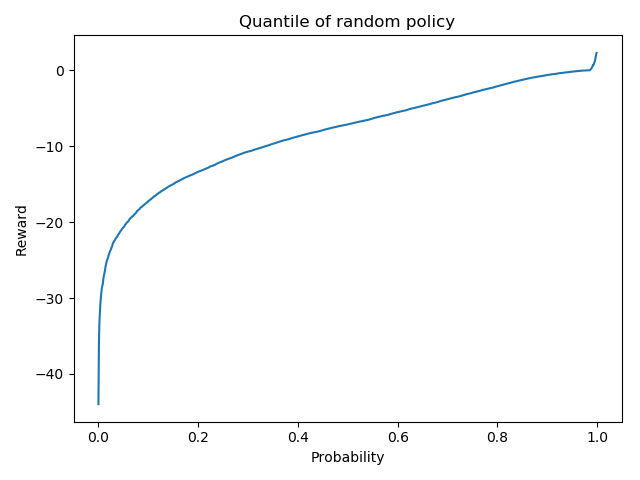
\includegraphics[height=4.5cm,width=6cm]{fig/Quantile_random.jpg}
    \end{minipage}
    \begin{minipage}[t]{0.5\textwidth}
    \centering
    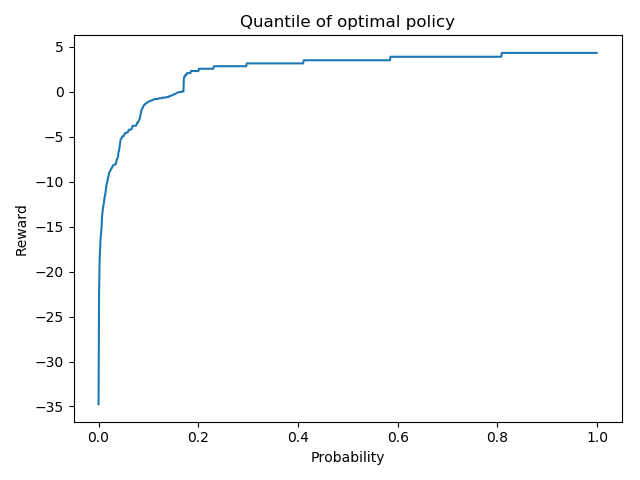
\includegraphics[height=4.5cm,width=6cm]{fig/Quantile_optimal.jpg}
    \end{minipage}
    \caption{Quantile of different policy}
    \end{figure}\\

    \item (5 Points) Using simulations, empirically estimate the probability that $S_{19}=21$ given that $S_8=18$ (the state above the goal) when running the uniform random policy. Describe how you estimated this quantity (there is \emph{not} a typo in this problem, nor an oversight).\\
    \textbf{Answer: }\\
    The empirical estimation of the probability that $S_{19}=21$ given that $S_8=18$ is about 0.03. The estimation begins with a start state in state 18, and the time step set to 8. Then the agent starts to take action randomly and interact with environment. If the agent enters into goal state, the trial end. At time step 19, stop the trail and see if the agent is in state 21.\\
\end{enumerate}
\end{document}
